%!TEX root = /Users/ede/Documents/Master/19_AS/Ausarbeitung/as-ausarbeitung.tex
\section{Motivation}

Durch erhöhte Bandbreiten und neue Techniken fand in den letzten Jahren eine hohe Zunahme an Multimedia Objekten im Internet statt. Die Multimedia Daten werden dabei sowohl auf privaten Webseiten als auch in sozialen Netzwerken wie Youtube\footnote{http://www.youtube.com}, Facebook\footnote{http://www.facebook.com} und auch das in diesem Paper näher behandelte Flickr\footnote{http://www.flickr.com} verfügbar gemacht.

Menschen suchen in der Regel Stichwort-basiert. Sie geben der Suchmaschine ein oder mehrere Schlüsselwörter, die in irgendeiner Beziehung zu den gesuchten Inhalten stehen. Um nun eine erfolgreiche Suche nach Multimedia Objekten zu ermöglichen, müssen die Medien nach \cite{collectiveKnowledge} reichhaltige Metadaten aufweisen, um eine Beziehung zwischen den Suchparametern und den durch die Suchmaschine indizierten Inhalten herzustellen. 

Die automatische Metadaten-Erstellung kostet nur wenig menschlichen Aufwand, nach \cite{combiningMultipleEvidence} ist es aber bisher nicht ausreichend für den praktischen Einsatz. Im Gegensatz zu reinem Text ist die automatische Extraktion von Metadaten aus Multimedia Objekten jedoch weitaus schwieriger. Die von Maschinen extrahierten Eigenschaften aus Multimedia Objekten sind zur Zeit noch auf einer zu niedrigen semantischen Ebene, so dass kein Bezug zu den Suchwörtern hergestellt werden kann. Der umgebende Text von Multimedia Daten, wie dies in Webseiten üblich ist, kann ebenfalls nur bedingt als Quelle für Metadaten genutzt werden, da dieser falsche oder unzureichende Angaben enthalten kann.

Somit ist die manuelle Generierung von Metadaten genauer und im Moment praktischer als die automatische Annotation. Weiterhin zeigt die rege Nutzung von sozialen Netzwerken, mit ihren Möglichkeiten der manuellen Annotation von Medien, dass diese Arbeit von den Autoren durchaus geleistet wird. Laut \cite{whyWeTag} sind die Gründe für das Taggen meist damit motiviert, dass die Urheber von Medien diese für die gesamte Nutzerschaft besser auffindbar machen wollen. 

Optimal wäre dabei die Verwendung von Ontologien zum Kennzeichnen und Einordnen der Objekte. Dieses Vorgehen ist jedoch nur für spezielle Fachgebiete möglich. Zunächst ist der Aufwand für die Erstellung solcher Ontologien sehr hoch und kostenaufwendig (siehe \cite{ontology_expensive1} und \cite{ontology_expensive2}). Aber auch die Verwendung vorgegebener und vor allem oft unbekannter Strukturen fällt den meisten Benutzern im Internet sehr schwer und erfordert relativ aufwendige Einarbeitung.

Eine vereinfachte Version der Generierung von Metadaten für Medienobjekte ist das \emph{Tagging} beziehungsweise \emph{Social Tagging}. Dabei geben die Nutzer einem Objekt frei gewählte Schlagwörter. Hierbei wird keine Taxonomie oder Ontologie vorgegeben und die Annotation wird aufgrund der einfachen Verfahrensweise von einer großen Anzahl von Menschen durchgeführt. Diese Art von Organisation wird auch \emph{Folksonomy} genannt.

Dabei gibt es eine Reihe von Problemen, die den Vorgang des Taggings erschweren beziehungsweise schlechte Ergebnisse liefern. Falsche, irrelevante und fehlende Tags führen jedoch zu schlechten Suchergebnissen.

\begin{itemize}
  \item \textbf{Synonyme:} Laut \cite{learningToTag} vergeben Menschen unterschiedliche Tags für die gleichen Objekte. Dies rührt daher, dass Menschen unterschiedliche Begriffe für die gleichen Objekte verwenden. Es ist gleichzeitig auch schwierig für den Benutzer alle zu einem Objekt passenden Begriffe zu finden.
  \item \textbf{Mehrdeutigkeit:} Benutzer verwenden allgemeine, mehrdeutige Begriffe, die ein Objekt nicht eindeutig beschreiben. Zum Beispiel könnte der Tag \emph{apple} die Annotation für eine Marke oder eine Frucht sein. Dabei wissen die Nutzer oft nicht mal etwas von der anderen Bedeutung oder erinnern sich nicht an die mit dem Objekt assoziieren Begriffe.
  \item \textbf{Semantischer Verlust:} Nicht alle Gegenstände und Informationen die in dem Medienobjekt enthalten sind werden annotiert.
  \item \textbf{Semantisches Rauschen:} Teilweise enthalten Medienobjekte Annotationen die keinen Zusammenhang zu dem Objekt besitzen.
\end{itemize}


Eine genaue Analyse und Klassifizierung der in Folksonomies enthaltenen Tags erfolgt in dem Kapitel \ref{sec:analyse_und_klassifikation}.

\subsection{Tag Ranking} % (fold)
\label{sub:tag_ranking}

% - mögliche Lösungen/Ansätze um Probleme zu reduzieren/beseitigen:
Um einige der oben genannten Probleme zu beseitigen oder wenigstens ihre Auswirkungen zu reduzieren, werden die Tags hinsichtlich ihrer Relevanz für das Medienobjekt untersucht und priorisiert. Es wird also ein Ranking, zu deutsch Einordnung oder Bewertung vorgenommen. Diese Ausarbeitung geht auf zwei solcher Tag-Ranking Algorithmen ein. Dabei werden unterschiedliche Ansätze gewählt, die sich hinsichtlich ihrer Herangehensweise und den Ergebnissen unterscheiden. Die den Verfahren vorangestellten Analysen werden in Kapitel \ref{sec:analyse_und_klassifikation} beschrieben, anschließend die Verfahren in Kapitel \ref{sec:tag_ranking_verfahren} im genauen vorgestellt und die Ergebnisse in Bezug auf Qualität und Performanz verglichen und bewertet.

\begin{figure}[htbp]
  \centering
    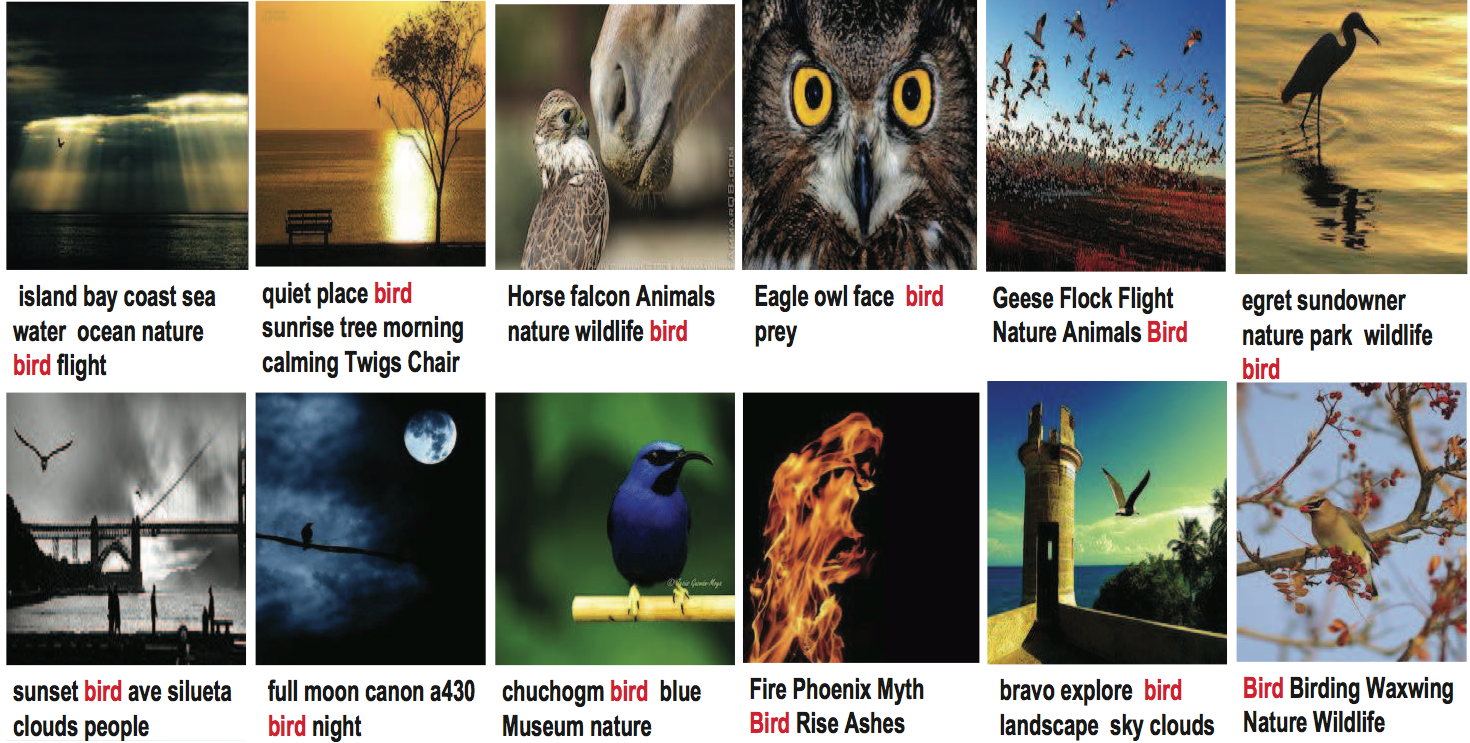
\includegraphics[height=0.5\textwidth]{images/bird_search_results_wide.png}
  \caption{Suchergebnisse bei einer Tag-basierten Flickr Suche nach \emph{bird} aus \cite{ranking}. Aus Platzgründen wird nur eine Auswahl von Tags pro Foto angegeben.}
  \label{fig:images_bird_search_results}
\end{figure}

Die aus der Anwendung der Algorithmen resultierende Vorteile liegen in besseren Suchergebnissen bei einer Stichwort basierten Suche und einem stark vereinfachten Tagging Prozess für den Benutzer sowie allgemein gesteigerter Relevanz der Tags. Abbildung \ref{fig:images_bird_search_results} veranschaulicht die Nachfrage für diese Art von Algorithmen. Zu sehen sind mehrere Bilder mit den annotierten Tags, die als Suchergebnis für das Suchwort \emph{bird} von Flickr ausgegeben werden. Man erkennt zunächst, dass die Tags nicht nach Relevanz für das jeweilige Bild sortiert sind und einige der Fotos nicht zur Anfrage passen.


% subsection tag_ranking (end)

\subsection{Anwendungsgebiete von Tags} % (fold)
\label{sub:anwendungsgebiete}

Wie oben schon erwähnt, werden Tags für die Suche nach Medienobjekten verwendet. Hierfür ist es besonders wichtig, dass die Tags Relevanzinformationen zu den assoziierten Medienobjekten aufweisen, um die Ergebnisse für den Benutzer in einer priorisierten Reihenfolge in Bezug zu der Suchanfrage auszugeben. Die ist vergleichbar mit den Suchergebnissen bei Google, die nach ihrer relativen Relevanz zu dem Suchbegriff und der objektiven Wichtigkeit der präsentierten Inhalte sortiert werden (siehe hierzu \cite{googlePageRank}).

Das zweite, wichtige Einsatzgebiet von Tags ist das Vorschlagen von Tags beim Tagging Prozess. Hierbei werden die gleichen Relevanzinformationen verwendet, um dem Benutzer die Annotations-Aufgabe zu erleichtern und dabei die Ergebnisse zu verbessern. Dabei werden auf Basis der bereits eingegebenen Tags weitere, damit assoziierte und relevante Tags vorgeschlagen, so dass der Benutzer diese nur noch auszuwählen braucht.
% Diese Ausarbeitung beschäftigt sich vor allem mit diesem Anwendungsfall und geht in den folgenden Kapiteln näher darauf ein.

%  TODO: rein oder raus:
 % - Vorschlagen von Gruppen für Photos

% subsection anwendungsgebiete (end)


% Fischer: Mir wäre dabei wichtig, dass Sie einen klaren Schwerpunkt setzen und ausgewählte Verfahren in die Tiefe behandeln.
% 
% Aufbau: 
%  - Kurze Einführung in das Gebiet des Taggings und Problembeschreibung
%  - Anwendungsgebiete der Ranking-Verfahren als Motivation
%  - Vorstellung der Ansätze um Bilder-Tags zu werten
%  -
